\section{Overview}

Building a Volumetric Simulator from scratch was a complex task that required the integration of various technologies and components. The most significant parts of the system are listed below, and we will discuss them in more detail in the following implementation sections.

\begin{itemize}[itemsep=-0.15em, label={}]
	\item \textbf{Simulator}: The simulator (\texttt{libvolsim.so}) is a shared library written in C++ that provides a graphical interface creating the illusion of a 3D display that can be interacted with.
	      \begin{itemize}[itemsep=-0.15em]
		      \item \textbf{Renderer Subsystem}: The rendering system is responsible for displaying the volumetric scene and the virtual objects within it. It uses OpenGL to render the scene based on user positional data from the tracking system, thus creating the illusion of 3D.
		      \item \textbf{Tracking Subsystem}: The tracking system monitors the user's hands and eyes within the scene. It employs machine learning models and a depth camera to track the user's head and eyes.
	      \end{itemize}
	\item \textbf{User Study CLI}: The User Study CLI (command-line interface) orchestrates the running of the simulator and stores the results of the user study in a MongoDB database. It also provides functionality to automatically analyse study data. This component is written in Python.
	\item \textbf{Build System}: The build system compiles the simulator and rendering system, as well as manages the execution of the user study. It uses Nix to handle dependencies and build the system in a declarative manner.
\end{itemize}

The user interacts with the \texttt{Study CLI}, to orchestrate running simulations by invoking the simulator's shared library \texttt{libvolsim.so}. The simulator returns its results/logs to the User Study CLI (in JSON format), which then stores the data in a MongoDB database. The User Study CLI can subsequently be used to analyse the results. A schematic of the system layout is shown in Fig~\ref{fig:system-layout}.

\begin{figureBox}[label={fig:system-layout}, width=1.0\linewidth]{Two examples of using our system}
    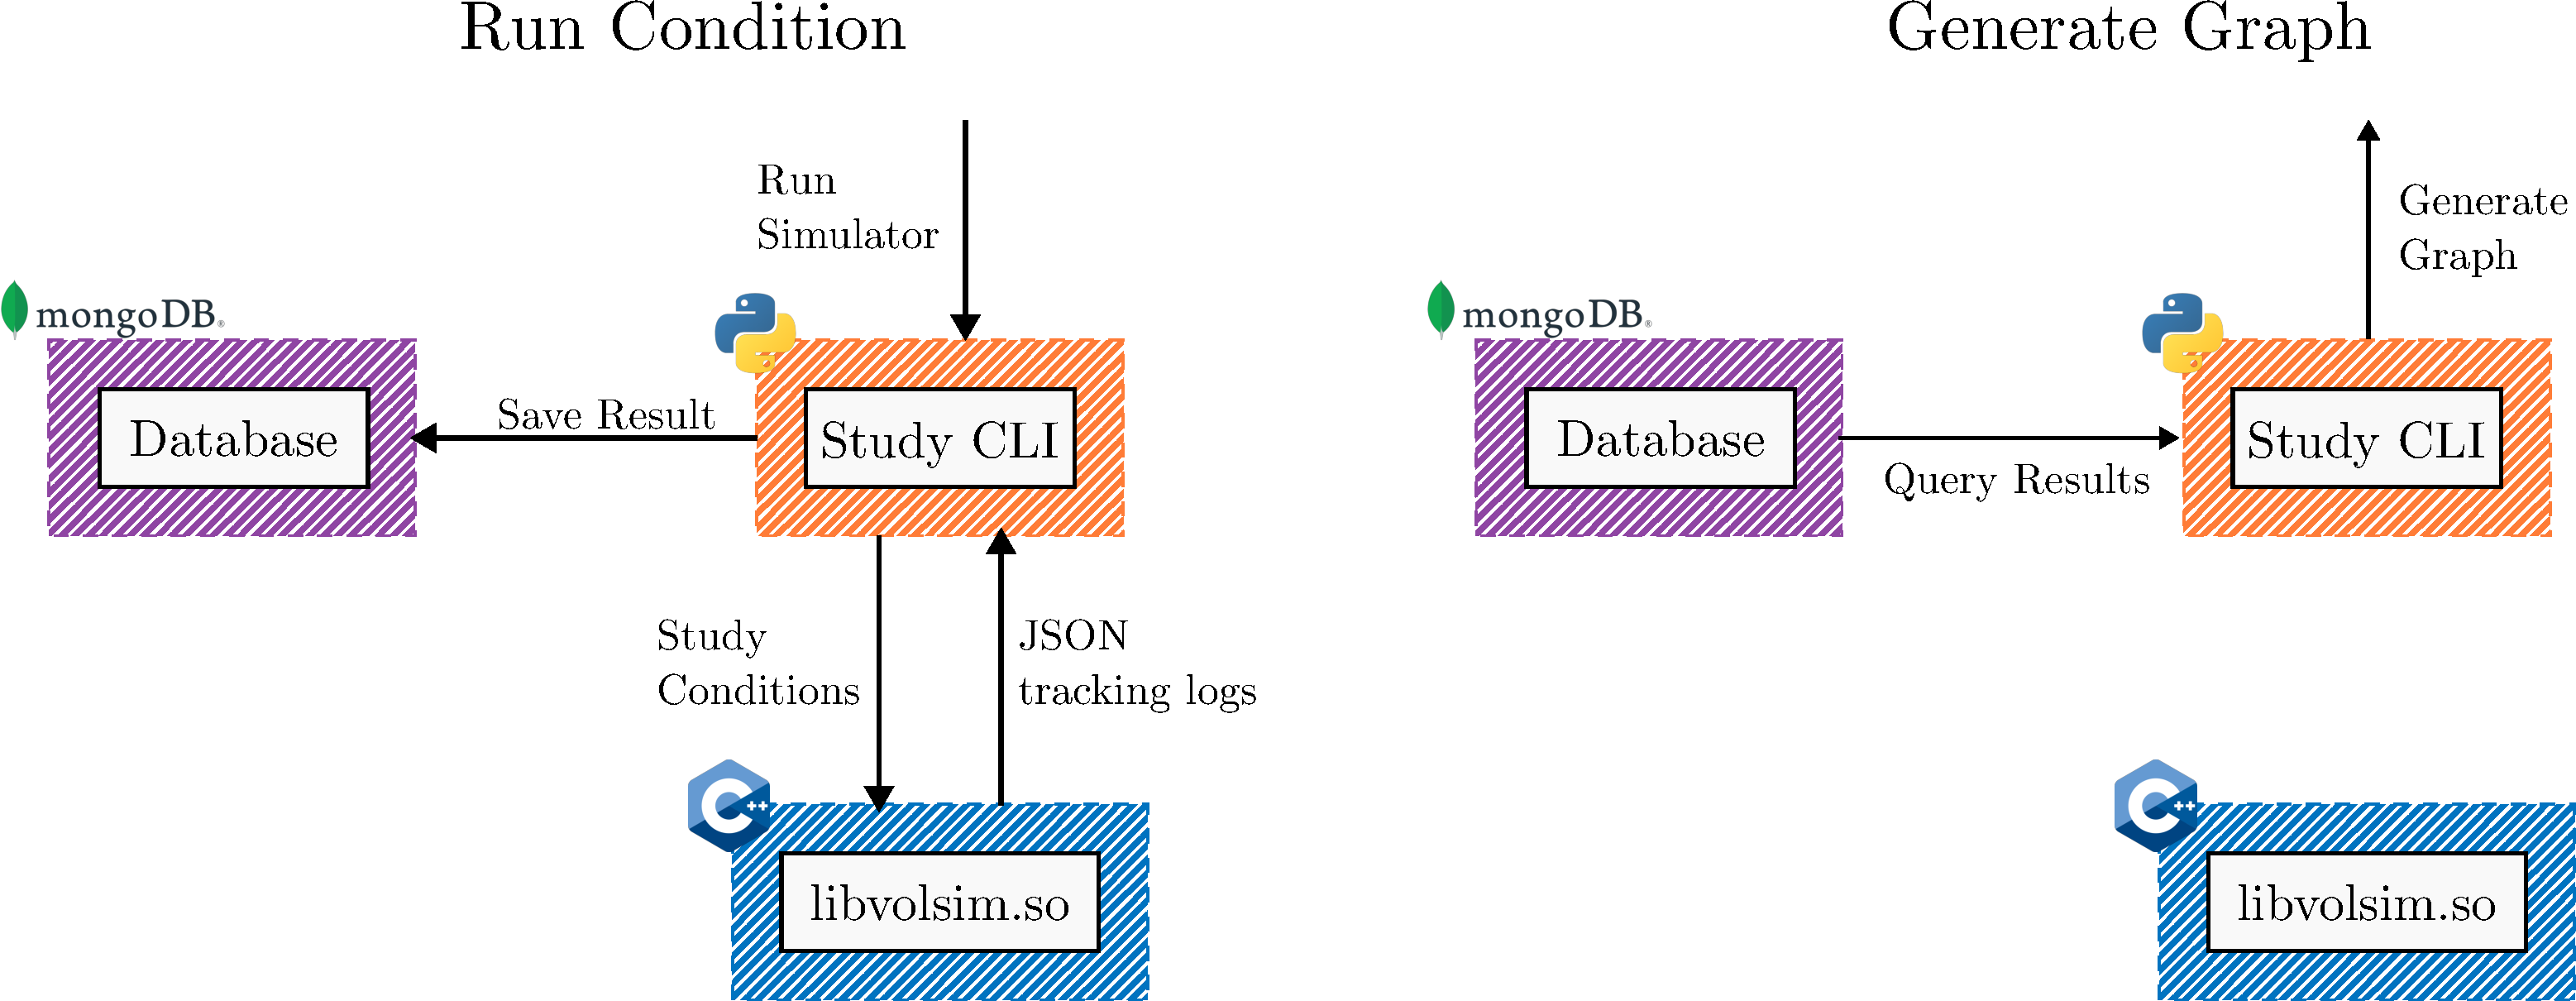
\includegraphics[width = 0.9\linewidth]{./implementation/figures/overall-system.pdf}
\end{figureBox}